\renewcommand{\tablename}{Tabla}
\chapter{Marco de Implementación} \label{Chapter:3}

\section{Capas Empleadas en las Arquitecturas Neuronales Convolucionales} \label{Chapter:Layers}

La forma más común de una arquitectura convolucional consiste en el apilamiento de algunas capas convolucionales y capas ReLU seguidas por capas de agrupación, repitiéndose este patrón hasta que la imagen de entrada disminuya espacialmente a un tamaño más reducido. En algunos puntos es común hacer transiciones a capas totalmente conectadas, de \textit{dropout} o capas de normalización. Sin embargo, en la práctica y en el 90\% de las aplicaciones el tipo de estructura es prácticamente intrascendente ya que las CNN son diseñadas o entrenadas desde cero tan sólo en ocasiones excepcionales \cite{CS231n}.

En otros términos, la disposición de la arquitectura convolucional más habitual, cuyas partes se describirán más detalladamente en los siguientes apartados, sigue el siguiente patrón:
\begin{align*}
    &\boxed{\text{Entrada}} \rightarrow \boxed{\boxed{\text{Capa Convolucional} \rightarrow \text{Capa ReLU}} \times \textbf{N} \rightarrow \text{Capa Pooling}} \times \textbf{M} \rightarrow \\ 
    & \boxed{\text{Capa Totalmente Conectada} \rightarrow \text{Capa ReLU}} \times \textbf{K} \rightarrow \boxed{\text{Capa Totalmente Conectada}}
\end{align*}

\subsection{Capa Convolucional}

\begin{figure}
    \centering
    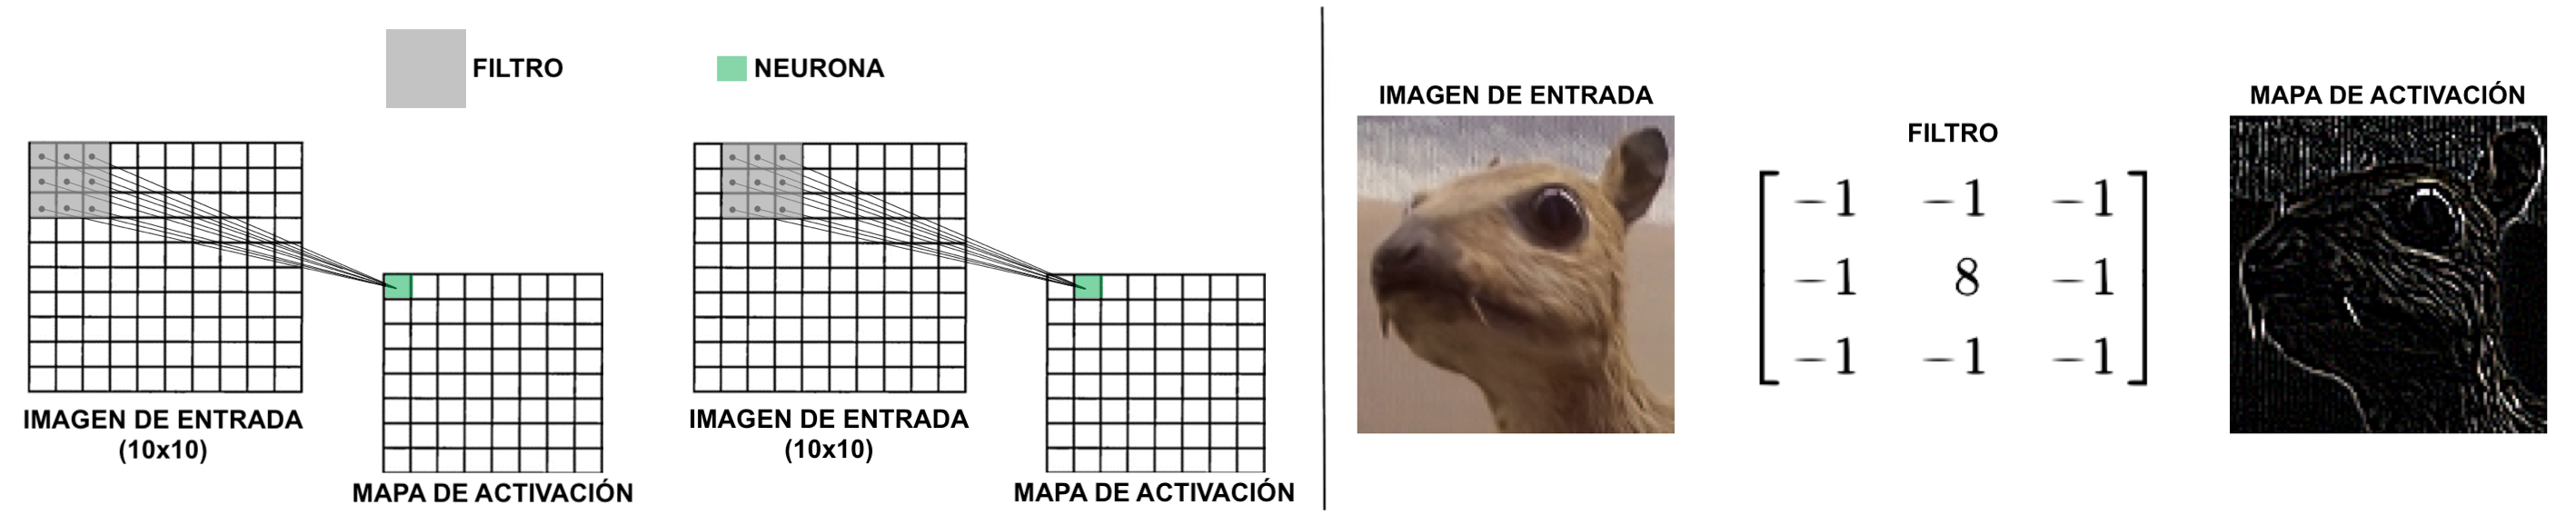
\includegraphics[width=\textwidth]{Images/ConvOperation.png}
    \caption{Las dos primeras iteraciones del proceso de convolución (izquierda) \cite{img:ConvOperation1} y resultado de la convolución de una imagen con una matriz detectora de bordes (derecha) \cite{img:ConvOperation2}.}
    \label{fig:ConvOperation}
\end{figure}

La capa convolucional es el componente básico de una CNN y sobre la que recae la mayor parte de las operaciones computacionales de la red. Su funcionamiento es análogo al de un filtro que discrimina toda la información que no sea relevante para el mapa de características o de activación. Durante el aprendizaje, cada uno de estos filtros se desliza a través del ancho y alto del volumen de entrada, calculándose la convolución entre el filtro y un área determinada del dato inyectado. De esta forma, se va generando un mapa de activación bidimensional que representa las respuestas del filtro en cada posición espacial, tal y como se puede advertir en la \autoref{fig:ConvOperation} y en la siguiente expresión:

\begin{align*}
    (I \ast K)_{x,y} &= \sum\limits_{i=0}^{h -1} \sum\limits_{j=0}^{w-1} K_{i,j} \cdot I_{x+i, y+j} \label{eq:1} \equiv \text{Mapa de Activación}\\
    \text{donde}~ 
    I &\equiv \text{imagen bidimensional de entrada,}\\
    K &\equiv \text{matriz de convolución o \textit{kernel} de dimensión $h\times w$}
\end{align*}

Esta compartición de pesos a lo largo de todo el campo visual es precisamente la que permita que todas las neuronas de una capa convolucional respondan de forma uniforme a una característica concreta, independientemente de su posición. Consecuentemente, la red aprenderá los filtros o pesos que se activan con algún tipo de singularidad visual, como bordes o manchas de algún color específico en las primeras capas o patrones enteros en las capas superiores. Finalmente, el volumen de salida se obtiene apilando los mapas de activación a lo largo de la dimensión de profundidad.

Por último, es necesario remarcar que la agrupación sucesiva de estas capas convolucionales tiene como fin la imposición de una arquitectura compuesta de filtros no lineales que, conforme aumenta la profundidad de la red, se van haciendo más globales y por lo tanto más sensibles a regiones más amplias del espacio de píxeles.

\subsection{Capa de Agrupación o de \textit{Pooling}}

La función principal de la capa de \textit{pooling} es la de reducir de forma progresiva el tamaño espacial (anchura y altura) de los mapas de activación para disminuir la cantidad de parámetros y la carga computacional de la red, controlando, de esta manera, el sobreaprendizaje. Esta operación también es conocida como reducción de muestreo ya que la síntesis de las características de una región implica la pérdida de información.

\begin{figure}
    \centering
    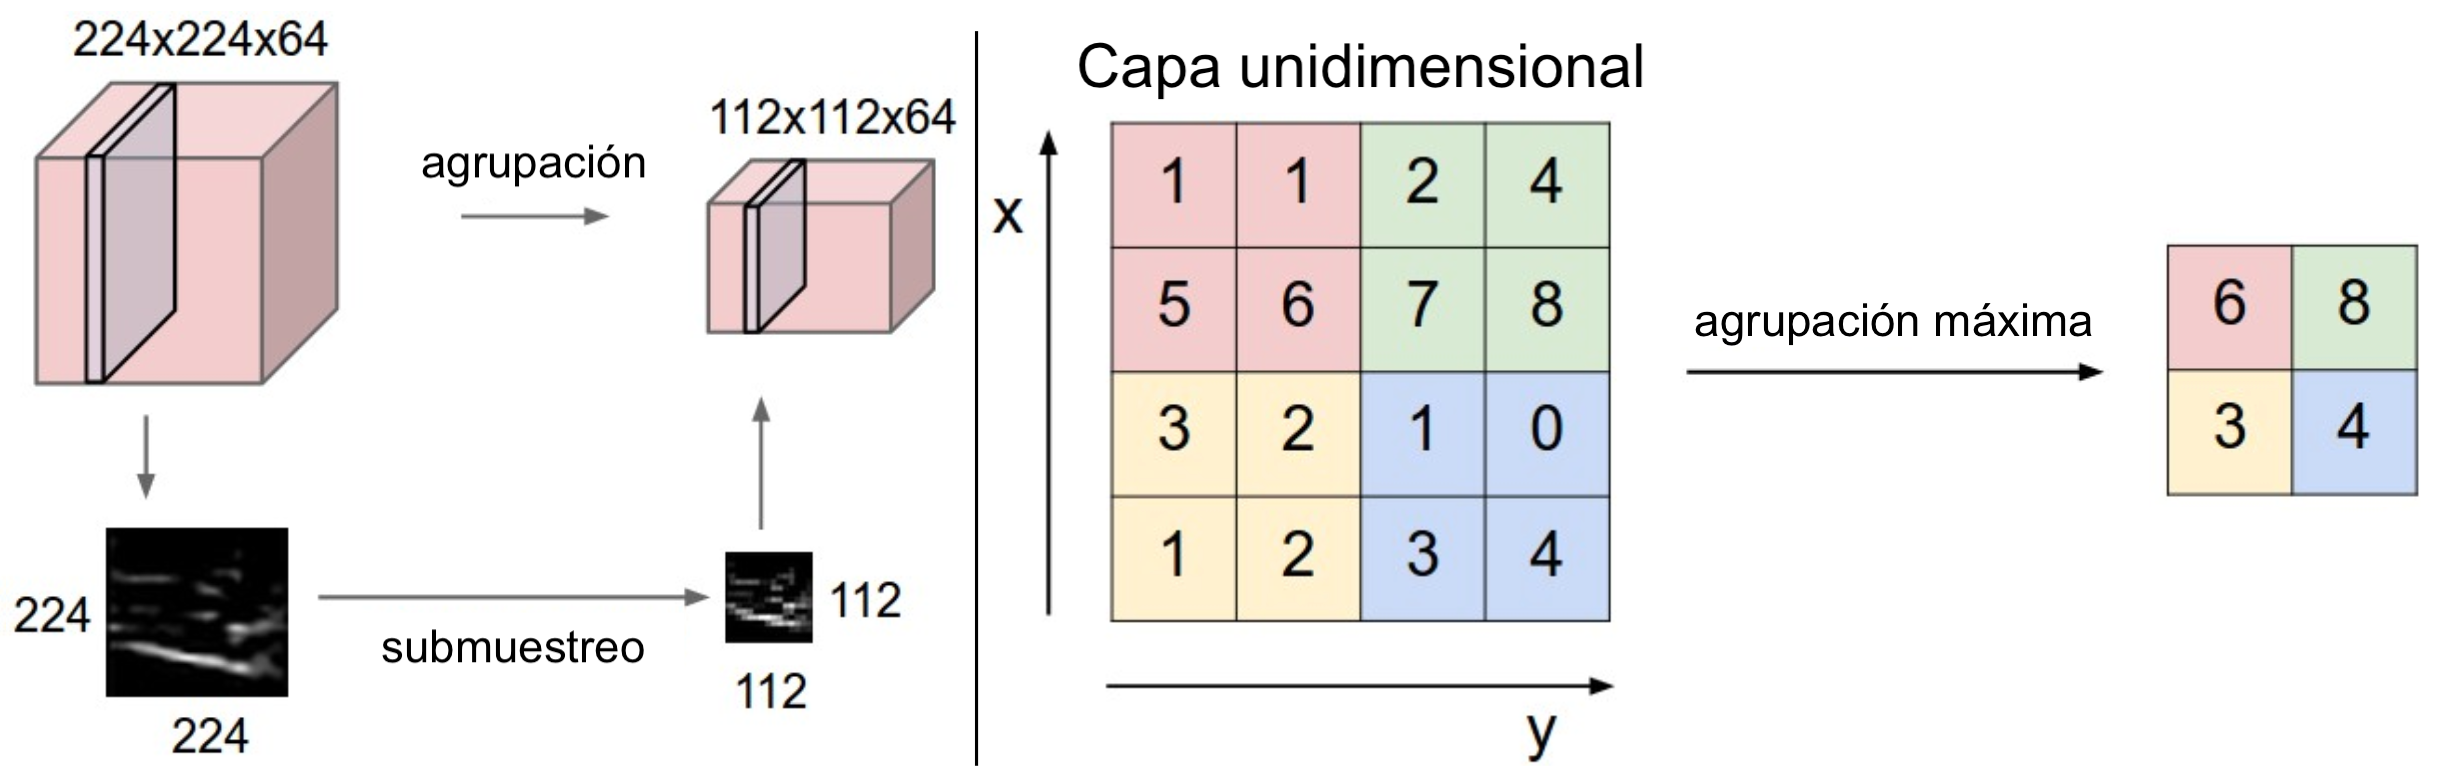
\includegraphics[width=\textwidth]{Images/Pooling.png}
    \caption{Operación de \textit{pooling} o de reducción de muestreo con un filtro de dimensión $2\times 2$ y paso de 2 unidades de píxel \cite{CS231n}.}
    \label{fig:Pooling}
\end{figure}

Existen varios esquemas posibles para realizar esta agrupación mediante la cual la imagen de entrada se divide en un conjunto de áreas que son reducidas a un único valor. Destacan los siguientes:
\begin{itemize}
  \item \textbf{Agrupación máxima (\textit{Max pooling})}. Toma el valor máximo de los píxeles de un bloque determinado.
  \item \textbf{Agrupación promedio (\textit{Average pooling})}. Calcula y toma el valor medio de un área de píxeles definida.
\end{itemize}

Tal y como se puede observar en la \autoref{fig:Pooling}, ambos métodos dan lugar a una reducción del tamaño de los datos por un factor igual a la dimensión de la ventana sobre la cual se opera o de destino, por lo que es común insertarlas periódicamente entre las sucesivas capas convolucionales en una arquitectura CNN \cite{CS231n}.

En la práctica y a pesar de que la agrupación promedio ha sido ampliamente explotada históricamente, la operación de agrupación máxima presenta un mejor funcionamiento al conservar de forma más eficaz las características más importantes de la imagen, haciendo que la red sea invariante a pequeñas transformaciones y distorsiones \cite{Pooling}.

\subsection{Capa Totalmente Conectada}

Una capa totalmente conectada es aquella cuyas neuronas, que no comparten conexiones dentro del mismo nivel, presentan enlaces absolutamente a cada una de las unidades de activación de la capa anterior, tal y como se ha visto en las redes neuronales convencionales (ANN) de la \autoref{Chapter:ANN}.

Dentro del contexto de las CNN, su principal función es la de realizar la clasificación en la última parte del modelo. Esto se consigue mediante una asignación de cada una de las dimensión de los datos de entrada a las clases de salida, obteniéndose de esta forma una decisión basada en la imagen completa insertada.

\begin{figure}
    \centering
    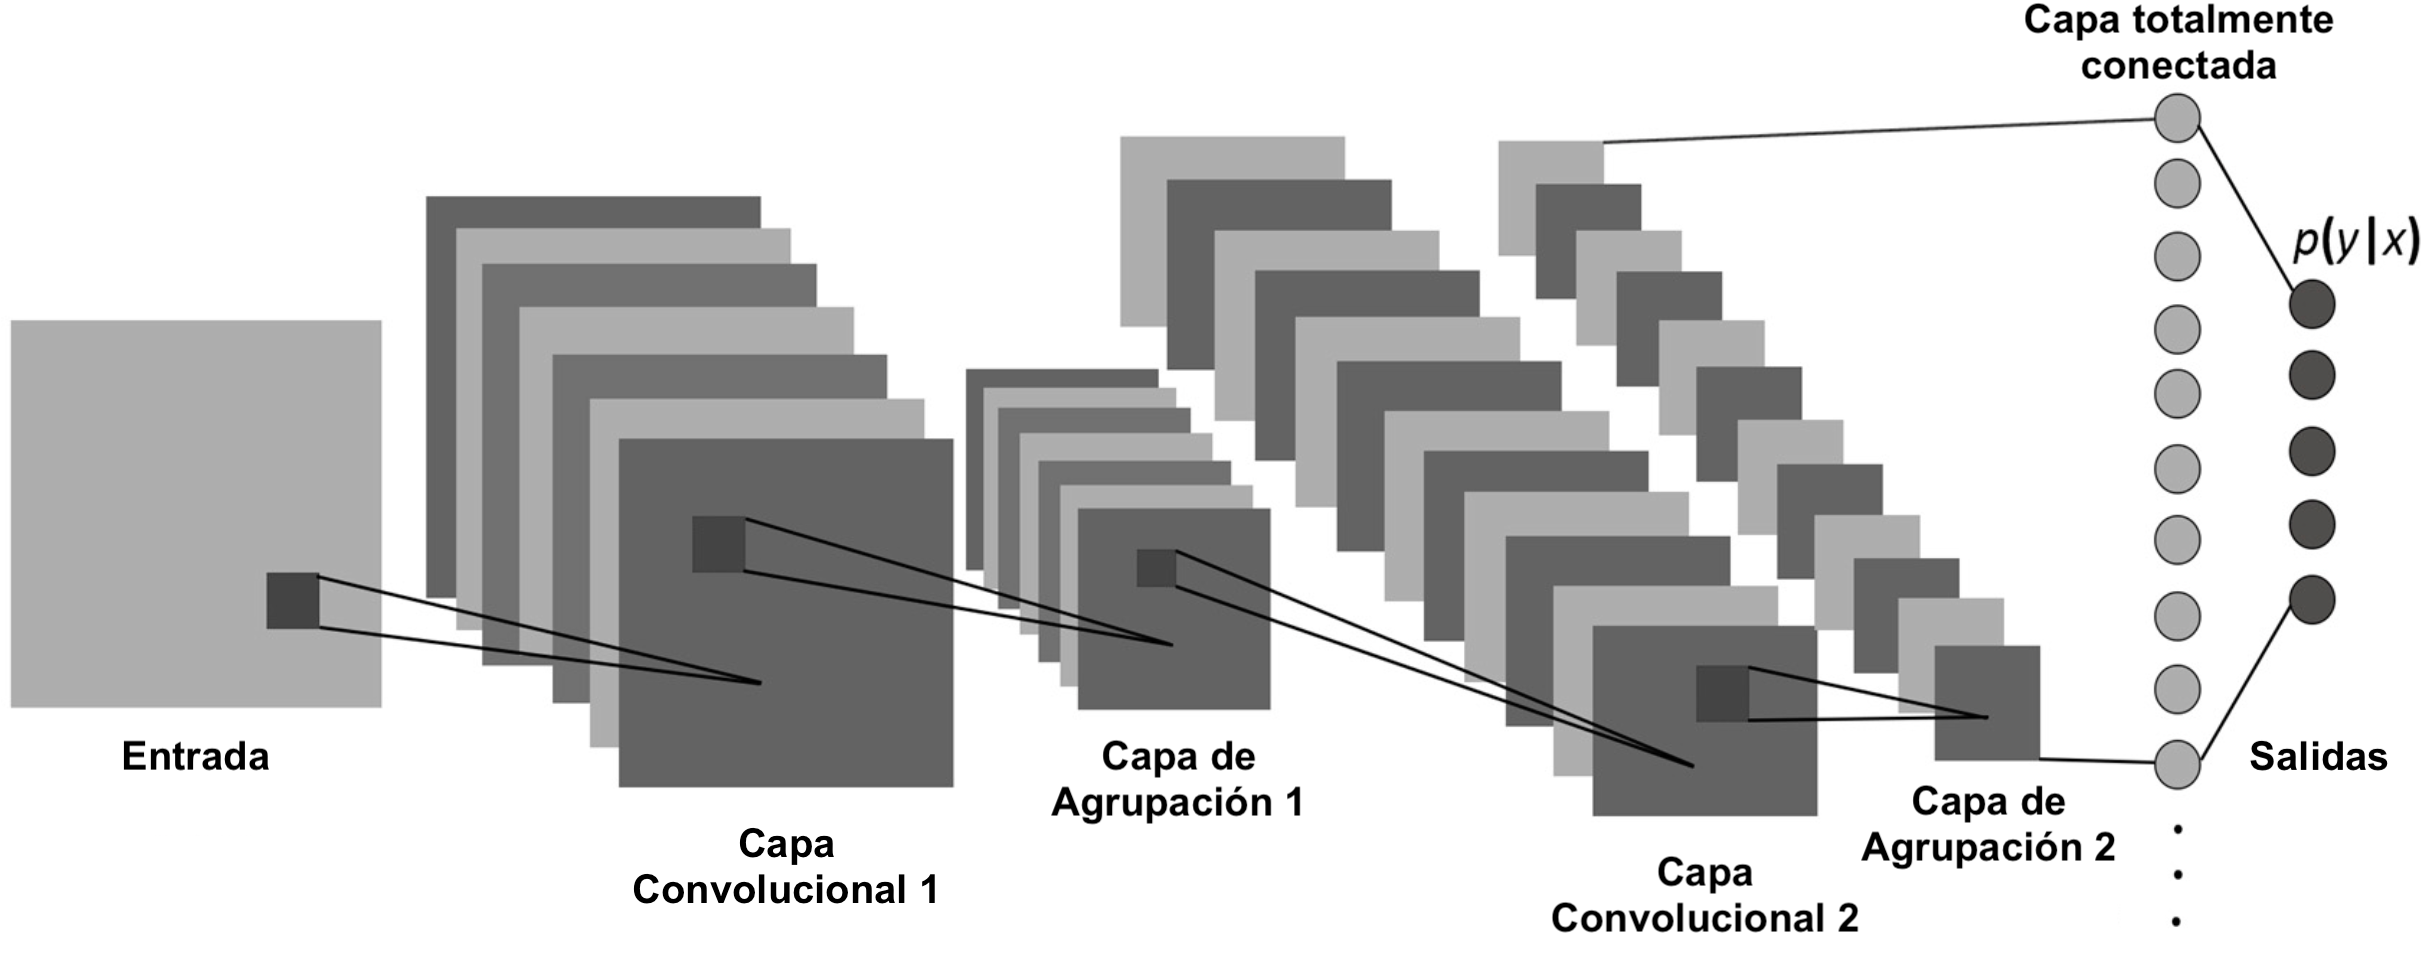
\includegraphics[width=\textwidth]{Images/CNN_architecture.png}
    \caption{Estructura simple de una CNN consistente en capas convolucionales, de agrupación y una capa totalmente conectada \cite{ArchitectureCNN}.}
    \label{fig:CNN_arch}
\end{figure}

En la \autoref{fig:CNN_arch} se puede observar tanto el empleo de la capa totalmente conectada en calidad de elemento clasificador, como una estructura típica simplificada de una CNN.

\hyphenation{ReLU} % evita partición de siglas
\subsection{Funciones de Activación: Unidad Lineal Rectificada (ReLU) y Función Exponencial Normalizada (SoftMax) }

La función de activación es una parte esencial de las arquitecturas de las ANN dado que tiene la capacidad de favorecer o perjudicar una determinada región del espacio de entrada de una unidad neuronal al controlar su umbral de activación.

En la actualidad, la función no lineal más popular es la unidad lineal rectificada (ReLU) \cite{DeepLearning}, representada en la \autoref{fig:ReLU} y cuya tarea es análoga a la de un rectificador de media onda:
\begin{align*}
    f(x) &= max(0, x) 
\end{align*}

\begin{figure}
    \centering
    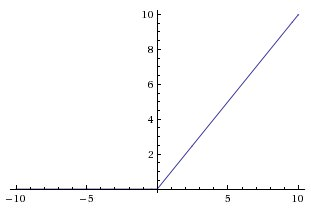
\includegraphics[scale=0.6]{Images/ReLU.png}
    \caption{Unidad Lineal Rectificada (ReLU) \cite{img:ReLU}.}
    \label{fig:ReLU}
\end{figure}

Anteriormente, en las redes neuronales se solían emplear funciones de activación más suaves (sigmoide, tangente hiperbólica, etc.), sin embargo, las ReLU generalmente permiten un aprendizaje mucho más rápido en redes profundas, acelerando el proceso incluso por un factor de 6 gracias a su forma lineal no saturante \cite{Krizhevsky}. Además, presentan un menor coste computacional ya que su implementación tan sólo requiere la aplicación de un umbral a una matriz de activación en cero, evitando, de esta manera, las costosas operaciones exponenciales de otras funciones.

A pesar de todo ello, mediante la función de activación ReLU no es posible computar las probabilidades de pertenencia de una entrada a unas determinadas clases de salida al ser los valores calculados por esta expresión difíciles de interpretar. En consecuencia, es necesario introducir e implementar una nueva función de activación, típicamente en la última capa de la arquitectura, para medir la compatibilidad de un conjunto de parámetros con respecto a las distintas categorías posibles. Esta habilidad, precisamente, es reunida por la función exponencial normalizada o SoftMax:
\begin{align*}
    p_i &= \frac{e^{f_{y_i}}}{\sum\limits_{j=1}^{N} e^{f_j}} & \forall \text{\space} i \in \text{1...N}\\
    \text{donde}~ 
    f_j &\equiv \text{elemento $j$-ésimo del vector de probabilidades}
\end{align*}

Tal y como puede observarse, esta función toma un vector N-dimensional y evalúa cada uno de sus elementos dentro del rango $[0, 1]$, cuya suma, además, pasa a ser la unidad, lo que proporciona un entorno especialmente adecuado para la interpretación probabilística en las tareas de clasificación multiclase.

\subsection{Capa de Normalización por Lotes}

La normalización por lotes es una técnica desarrollada para mitigar el efecto de una inicialización desacertada de los pesos de las redes neuronales. Se consigue al forzar explícitamente a las activaciones de la capa previa a asumir una distribución unitaria gaussiana en cada lote al comienzo del entrenamiento.

En comparación con los modelos convencionales de reconocimiento de imágenes, la inclusión de este procedimiento da lugar a que se alcancen los mismos resultados con un número de iteraciones de entrenamiento 14 veces menor \cite{BatchNormalization}. Esto es gracias a que la introducción de esta capa posibilita el empleo de tasas de aprendizaje mucho más altas, a la vez que permite eliminar la compleja labor de diseñar un inicializador adecuado.

El pseudocódigo de este proceso viene descrito más detalladamente en el \autoref{alg:BatchNormalization}.

\begin{algorithm}
\caption{Normalización por Lotes \cite{BatchNormalization}}
\label{alg:BatchNormalization}
\begin{algorithmic}[1]
    \Function{BatchNormalization}{datos, red}
        \State \VARIABLES $\gamma, \beta$ \textcolor{blue}{\footnotemark[1]} \Comment{Parámetros por aprender}
        \Repeat
            \ForEach{lote $\mathfrak{B} = \lbrace x_{1 ... m}\rbrace$ \IN datos}
                \State $\mu_\mathfrak{B} \gets \frac{1}{m}\cdot \sum\limits_{i=1}^{m} x_i$ \Comment{Promedio del lote}
                \State $\sigma_\mathfrak{B}^{2} \gets \frac{1}{m}\cdot \sum\limits_{i=1}^{m} (x_i - \mu_\mathfrak{B})^2 $ \Comment{Varianza del lote}
                \State $\hat{x}_i \gets \frac{x_i - \mu_\mathfrak{B}}{\sqrt{\sigma_\mathfrak{B}^{2} + \epsilon}}$\Comment{Normalización}
                \State $y_i = \gamma \cdot \hat{x}_i + \beta$\Comment{Escalado y desplazamiento}
            \EndFor
        \Until todos los lotes de datos normalizados
        \State \Return $y$
    \EndFunction
\end{algorithmic}
\textcolor{blue}{\footnotesize{\\ $^1$ La tarea de los parámetros $ \gamma $ y $\beta$ es la de mantener la media y la varianza a unos valores preestablecidos.}}
\end{algorithm}

En la práctica, estas capas son insertadas inmediatamente después de las capas totalmente conectadas o convolucionales y antes de las funciones no lineales. Además, es una técnica muy utilizada actualmente ya que las redes neuronales que las explotan son significativamente más robustas a una inicialización incorrecta \cite{CS231n}.

\subsection{Capa de \textit{Dropout}}

La operación de \textit{Droput} es una técnica que permite evitar el sobreaprendizaje, proporcionando una forma de combinar, aproximadamente y de forma exponencial, distintas arquitecturas neuronales de un mismo modelo de manera eficiente \cite{Srivastava}. 

\begin{figure}
    \centering
    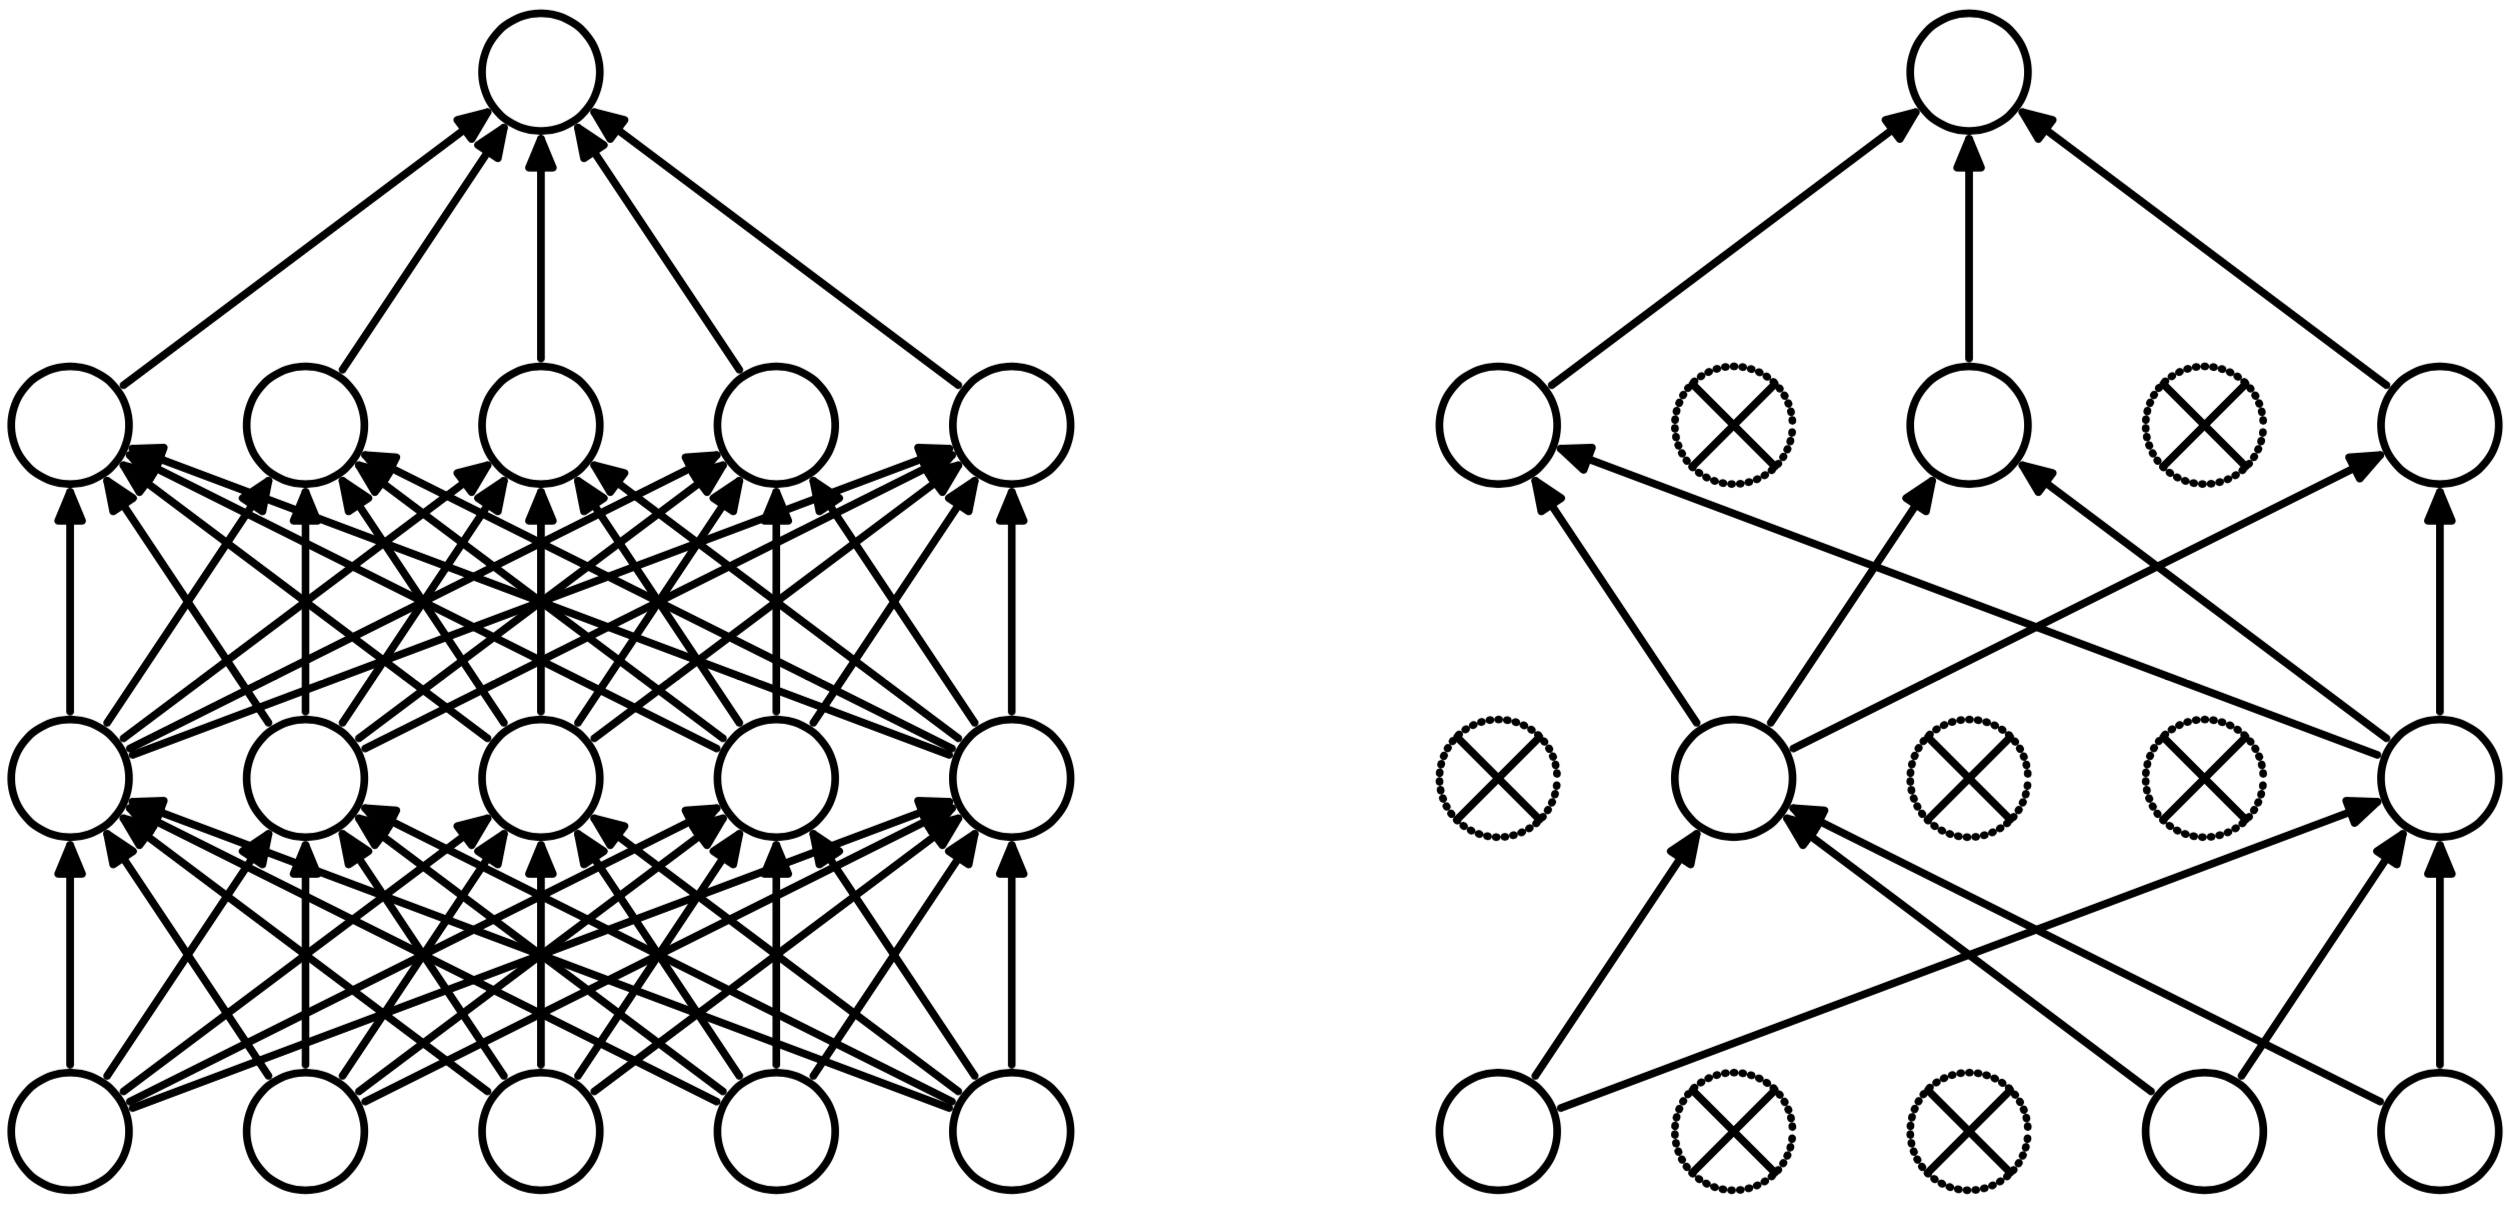
\includegraphics[scale=0.25]{Images/Dropout.png}
    \caption{Red neuronal estándar con 2 capas ocultas (izquierda) y red de mismas características a la que se le ha aplicado la operación de \textit{Dropout} (derecha) \cite{Srivastava}.}
    \label{fig:Dropout}
\end{figure}

Su funcionamiento es bastante simple, ya que consiste en el apagado aleatorio, en cada una de las iteraciones del proceso de aprendizaje, de una serie de unidades neuronales con una probabilidad de $1 - p$. Cabe destacar que esta red reducida mantiene los pesos originales de las neuronas desactivadas, eliminándose, tan sólo, las conexiones entrantes y salientes, tal y como se muestra en la \autoref{fig:Dropout}.

Esta técnica principalmente minimiza el impacto de las neuronas con activaciones dominantes, lo que proporciona a su vez un entorno de mayor independencia entre las distintas unidades durante el entrenamiento. Asimismo, su empleo también consigue mejorar significativamente la velocidad de entrenamiento al reducirse el número de interacciones entre los nodos, lo que además da lugar a una respuesta más generalizada por parte de la arquitectura ante la inserción de datos nuevos.

En definitiva, es un procedimiento muy básico que presenta un funcionamiento excelente para combatir el sobreaprendizaje sin la necesidad de introducir más regularizadores \cite{CS231n}.

\section{Keras y TensorFlow}

Keras es una Interfaz de Programación de Aplicaciones (API) de redes neuronales de alto nivel, escrita en Python y capaz de ejecutarse sobre TensorFlow. Esta última, por su parte, es una biblioteca de software de código abierto desarrollada por el departamento de inteligencia artificial de Google para la computación numérica de alto rendimiento con la capacidad de implementarse y ejecutarse utilizando múltiples Unidad de Procesamiento Central (CPUs), Unidad de Procesamiento Gráfico (GPUs) y Unidad de Procesamiento Tensorial (TPUs).

La decisión del empleo de estas dos herramientas, concretamente de Keras sobre TensorFlow, radica en que su combinación proporciona un entorno modular, extensible y fácil de usar, ofreciendo un gran número de utensilios de aprendizaje profundo. En este contexto, Keras facilita tanto las herramientas para desarrollar las arquitecturas neuronales, como el medio y los métodos para entrenar los modelos. Además, en lo que respecta al campo del reconocimiento visual, pone a disposición de la comunidad una gran variedad de modelos preentrenados con distintas bases de datos y que pueden emplearse para la predicción, la extracción de características y la afinación de otros sistemas que planteen problemas similares. De hecho, la existencia de estos modelos, que son reconocidos como los estados del arte dentro de su ámbito, simplifica notablemente la implementación de técnicas como la transferencia de aprendizaje.

\section{Transferencia de Aprendizaje}

El aprendizaje por transferencia consiste en la reutilización del conocimiento adquirido durante la resolución de un problema concreto y su posterior aplicación como parte de la solución a uno nuevo, de diferente índole, pero estrechamente relacionado.

Esta forma de abordar los problemas de aprendizaje profundo se debe a que para conseguir unos resultados meramente aceptables es necesario un modelo complejo, el cual, para un entrenamiento desde cero, requiere tanto de considerables recursos (GPUs), como de tiempo (días e incluso semanas de entrenamiento, dependiendo del modelo y del número de GPUs utilizadas). De hecho, en la práctica, el entrenamiento de una red reuronal convolucional completa con una inicialización aleatorio o pseudoaleatoria es realizada por un número reducido de personas, ya que es relativamente raro tener un conjunto de datos de tamaño suficiente con los recursos requeridos para manejarlos \cite{CS231n}.  

Existen dos escenarios principales del aprendizaje transferido:
\begin{itemize}
  \item \textbf{Extracción de características fijas}. Se emplea una CNN entrenada previamente con una base de datos determinada y a la que se le elimina la última capa totalmente conectada, introduciéndose en su lugar un clasificador instruido con un nuevo conjunto de datos. De esta forma, la red original tan sólo funciona como un extractor de características fijo, mientras que el predictor insertado posibilita una clasificación particularizada.
  \item \textbf{Afinación de modelos}. En esta ocasión no sólo se remplaza y reentrena el clasificador de la parte superior de la CNN con el nuevo conjunto de datos, sino que también son ajustados los pesos de la red inicial mediante la continuación del proceso de retropropagación. Asimismo, es posible afinar un número determinado de capas, generalmente las superiores, manteniendo fijos los pesos de las demás. Esto es especialmente útil para evitar el sobreaprendizaje al ser las CNN sensibles a características más genéricas en los niveles iniciales y más específicas en los finales.
\end{itemize}

En el contexto de este proyecto, se va a explotar principalmente la afinación de arquitecturas convolucionales dada la disponibilidad de una cantidad aceptable de imágenes de expresiones faciales, así como de una serie de modelos preentrenados y estrechamente relacionados con el ámbito del reconocimiento de emociones. De hecho, transferir modelos y luego afinarlos da como resultado redes que ofrecen una mejor generalización en comparación con aquellas que son entrenadas directamente con el conjunto de datos disponible \cite{TransferLearning}.

\section{Google Cloud Plataform}

Google Cloud Platform es una plataforma que ofrece un conjunto de servicios modulares de computación en la nube, entre los que destacan el almacenamiento de datos, el análisis de datos y el aprendizaje automático. Dentro de este último punto, se van a utilizar básicamente tres herramientas: \begin{itemize}
  \item \textbf{Cloud Machine Learning Engine}. Es un servicio que proporciona un entorno de implementación de modelos complejos de aprendizaje automático, permitiendo ejecutar aplicación desarrolladas sobre TensorFlow con ciertas alteraciones. Concretamente, mediante este servicio es posible realizar tareas previas de procesado de datos, entrenar modelos de aprendizaje profundo y evaluar sistemas existentes.
  
  La GPU empleada por este servicio y la única ofrecida actualmente es la NVIDIA Tesla K80.
  \item \textbf{Compute Engine -- Cloud Datalab}. Este producto permite desarrollar proyectos en máquinas virtuales escalables de alto rendimiento y ejecutarlos en las infraestructuras de Google. El medio específico que se utiliza es Cloud Datalab, que es una herramienta interactiva que posibilita la exploración, el análisis y la visualización de datos, así como el desarrollo de modelos de aprendizaje automático en \textit{notebooks} con Python y TensorFlow.
  
  En este caso se dispone de una GPU más potente, la NVIDIA Tesla P100, que permite superar las limitaciones de memoria impuestas por el servicio Cloud Machine Learning Engine.
  \item \textbf{Cloud Storage}. Es el sistema de almacenamiento de la plataforma Google Cloud. Abarca tareas relacionadas tanto con el suministro, el archivado y el análisis de datos, como con el aprendizaje automático. En este proyecto su utilización se centra en el guardado de los puntos de control de los modelos, así como en el almacenamiento de los registros y métricas que permiten analizar el estado del entrenamiento o del aprendizaje en tiempo real. 
\end{itemize}

\begin{table}
\centering
\label{Table:GPU}
\begin{tabular}{c|c|c|c|c|}
    \cline{2-5}
    & \textbf{Memoria} & \textbf{Núcleos} & \textbf{\begin{tabular}[c]{@{}c@{}}B/W \\ Memoria\end{tabular}} & \textbf{\begin{tabular}[c]{@{}c@{}}Memoria\\ disponible\end{tabular}} \\ \hline
    \multicolumn{1}{|c|}{\textbf{\begin{tabular}[c]{@{}c@{}}NVIDIA \\ Quadro K4000\end{tabular}}}   & 3 GB GDDR5    & 768 & 134 GB/s    & -- \\ \hline
    \multicolumn{1}{|c|}{\textbf{\begin{tabular}[c]{@{}c@{}}NVIDIA\\ Tesla K80\end{tabular}}}       & 12 GB GDDR5   & 2496 & 240 GB/s   & 1 -- 52 GB \\ \hline
    \multicolumn{1}{|c|}{\textbf{\begin{tabular}[c]{@{}c@{}}NVIDIA\\ Tesla P100\end{tabular}}}      & 16 GB HBM2    & 3584 & 732 GB/s   & 1 -- 104 GB \\ \hline
\end{tabular}
\caption{Comparación entre las GPUs empleadas}
\end{table}

El uso de esta plataforma para la afinación de los modelos propuestos tiene como finalidad la reducción de forma abrupta del tiempo de aprendizaje. De hecho, empleando las herramientas anteriormente descritas se ha corroborado personalmente un incremento de la velocidad de entrenamiento de entre 6 y 7 veces con respecto a la utilización de un computador con una GPU NVIDIA Quadro K4000 (gama alta del año 2013) y de hasta 30 veces en comparación con el desempeño obtenido por un computador portátil personal que carece de unidades de procesamiento gráfico. Las comparaciones entre estos equipos puede verse en la \autoref{Table:GPU}.

Por último, hace falta mencionar que la elección de Google Cloud Plataform en favor de otros servicio de computación en la nube, como Amazon Web Services o Microsoft Azure, ha estado motivada principalmente por razones económicas y de soporte ya que Google es el proveedor que ofrece la mayor variedad de servicios dentro de su periodo de prueba gratuito.

\section{Bases de Datos}

En el proceso de desarrollo del sistema de reconocimiento de emociones de este proyecto se emplean, directa o indirectamente, tres tipos de bases de datos distintas. Por un lado se hace uso de los conjuntos de datos ImageNet \cite{ImageNet} y VGGFace2 \cite{VGGFace2}, que son precisamente los aprendidos por los modelos preentrenados ofrecidos por Keras. Por el otro destaca FER-2013 \cite{FER-2013}, que es la base de datos mediante la cual se va a realizar el afinamiento de los sistemas iniciales para dotarlos de la capacidad de reconocer expresiones faciales.

\subsection{ImageNet}

ImageNet es una base de datos visual enfocada en la investigación de \textit{software} para el reconocimiento de objetos visuales y compuesta por tres subconjuntos de datos: entrenamiento (1.2 millones de imágenes), validación (50000 imágenes) y evaluación (100000 imágenes). Estas fotografías, recopiladas de Flickr y otros motores de búsqueda, están etiquetadas a mano indicando la presencia o ausencia de 1000 categorías de objetos, los cuales abarcan ámbitos tan diversos como razas de perro, especies de plantas u hongos, distintos objetos cotidianos o personas.

Esta amplitud, heterogeneidad y no superposición de clases es la que ha convertido precisamente a ImageNet en el punto de referencia para los algoritmos de clasificación de imágenes, dominados por las redes neuronales convolucionales y las técnicas de aprendizaje profundo desde 2012. Por esta razón, de hecho, gran parte de los modelos que mejor rendimiento han obtenido con esta base de datos se han incluido en la biblioteca de Keras.

\subsection{VGGFace2}

Esta base de datos contiene 3.31 millones de imágenes faciales de 9131 sujetos célebres, con un promedio de 362.6 fotografías por individuo y con una gran diversidad de poses, de edades, de iluminación, de etnias y de profesiones. Todo el conjunto de datos se divide en un grupo de entrenamiento de 8631 individuos y en uno de pruebas de 500 individuos. Además, VGGFace2 proporciona anotaciones que permiten la evaluación de los distintos sujetos en dos escenarios diferentes: coincidencia de rostros de diferentes poses y coincidencia de rostros de diferentes edades.

\subsection{FER-2013} \label{Chapter:FER-2013}

\begin{figure}
    \centering
    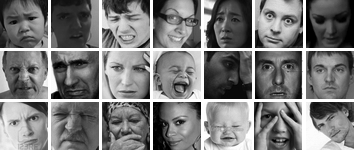
\includegraphics{Images/FER-2013.png}
    \caption{Imágenes extraídas de la base de datos FER-2013 \cite{Pramerdorfer}.}
    \label{fig:FER-2013}
\end{figure}

FER-2013 es la base de datos estáticos de expresiones faciales de mayor relevancia disponible públicamente. Consta de 35887 representaciones en escala de grises adquiridas de entornos no acondicionados expresamente con una resolución de $48 \times 48$ píxeles. Este conjunto reúne rostros de distinta naturaleza en términos de edad, orientación de la cara, etnia y género, tal y como puede observase en la \autoref{fig:FER-2013} y está dividido en tres subgrupos: entrenamiento, validación y evaluación con 28709, 3589 y 3589 muestras respectivamente. Asimismo, cada una de las imágenes está etiquetada con respecto a la expresión manifestada por el sujeto en la fotografía.

\begin{table}
\centering
\begin{tabular}{c|c|c|c|c|c|c|c|}
    \cline{2-8}
    & \textbf{Ira} & \textbf{Asco} & \textbf{Miedo} & \textbf{Alegría} & \textbf{Tristeza} & \textbf{Sorpresa} & \textbf{Neutral} \\ \hline
    \multicolumn{1}{|c|}{\textbf{\begin{tabular}[c]{@{}c@{}}Núm. de\\ imágenes\end{tabular}}} & 4953 & 547 & 5121 & 8989 & 6077 & 4002 & 6198 \\ \hline
\end{tabular}
\caption{Número de imágenes por cada expresión facial de la base de datos FER-2013.}
\label{Table:FER-2013}
\end{table}

En la \autoref{Table:FER-2013} se muestra la cantidad de imágenes en esta base de datos de las seis expresiones básicas y la expresión neutral. Como puede advertirse, hay un desequilibrio de clases notable, hecho que va a influir negativamente en el desempeño del modelo, especialmente para las emociones con menor representación.  

Por último, cabe destacar que la precisión humana sobre este conjunto de datos es aproximadamente de $65\pm 5\%$ \cite{FER-2013_human_acc}.

\section{Aumento de datos}

En el campo del aprendizaje profundo, donde el tamaño de las bases de datos tiene una gran influencia en el resultado final, el aumento de datos se usa a menudo para expandir tanto los resultados como la versatilidad del entrenamiento. En cuanto a las técnicas existentes, éstas pueden agruparse en tres tipos principales:

\begin{itemize}
    \item \textbf{Aumento a través de Transformaciones Geométricas}. Se generan nuevas imágenes mediante transformaciones lineales (rotación, traslación, escalado, etc.) que preservan la clase o etiqueta de la representación original.
    \item \textbf{Aumento Guiado por Atributos (AGA)} \cite{AGA}. El conjunto de entrenamiento es aumentado mediante descriptores de características en lugar de imágenes. Específicamente, esta técnica aprende a sintetizar ciertas propiedades guiada por los valores estimados de un conjunto de atributos, como la profundidad o la pose.
    \item \textbf{Aumento mediante Redes Generativas Antagónicas (GAN)} \cite{GAN}. A partir de una distribución de datos inicial, estas redes son capaces de producir nuevas representaciones de forma artificial gracias a la imitación de ciertas características de alto nivel extraídas de las imágenes originales.
\end{itemize}

De esta forma y teniendo en cuenta las limitaciones de la mayoría de las bases de datos, se hace evidente que el empleo de estas técnicas puede dar lugar a mejoras considerables de los resultados. Asimismo, en el contexto de la clasificación de imágenes de expresiones faciales, donde los datos, en la mayoría de los casos, son inadecuados o insuficientes y la distribución de clases desequilibrada, parece resultar especialmente adecuado el empleo de las redes generativas y de las transformaciones geométricas para mejorar el conjunto de entrenamiento.

\subsection{Redes Generativas Antagónicas}

Las redes generativas antagónicas son una clase de algoritmos de inteligencia artificial desarrolladas por Ian Goodfellow en 2014 y utilizadas en el aprendizaje automático no supervisado \cite{GAN}. Están formadas por un sistema de dos redes neuronales que compiten entre ellas y cuyo funcionamiento es análogo al algoritmo recursivo o método de decisión \textit{minimax} restringido para dos individuos, el cual consiste en elegir el mejor movimiento para ti mismo suponiendo que tu contrincante escogerá el peor para ti. 

\begin{figure}
    \centering
    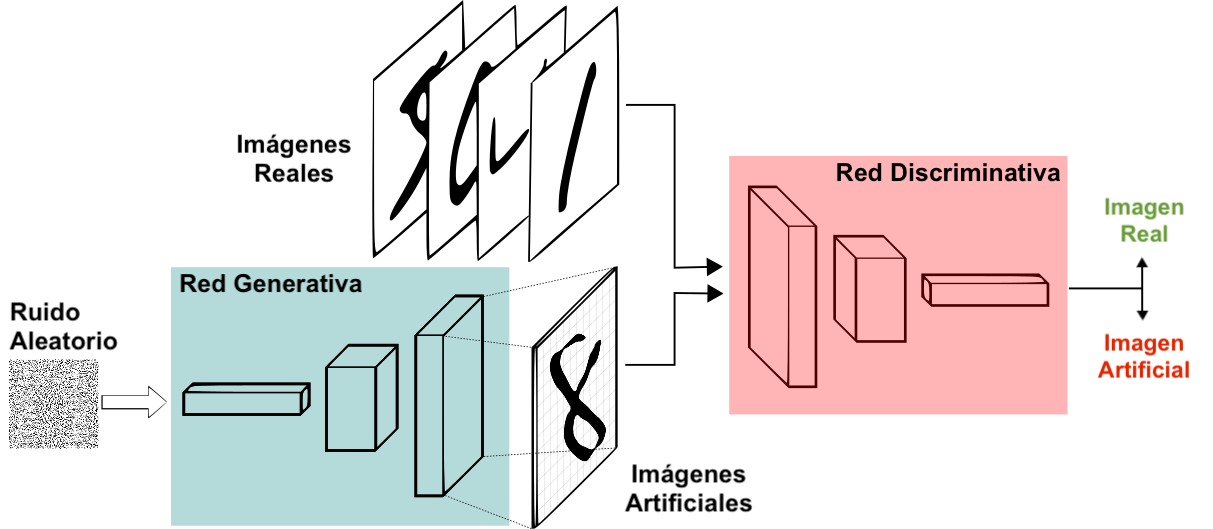
\includegraphics[width=\textwidth]{Images/GAN.png}
    \caption{Arquitectura de una Red Generativa Antagónica (GAN) \cite{img:GAN}.}
    \label{fig:GAN}
\end{figure}

En la \autoref{fig:GAN} se muestra la estructura de este tipo de redes caracterizadas por integrar dos modelos diferentes, uno generativo y otro discriminativo, que además, son entrenados simultáneamente. La representación matemática del funcionamiento de esta arquitectura es la siguiente:

\begin{align}
    \underset{G}{min} \ \underset{D}{max} \ \mathcal{V}(D, G) &= \underbrace{\mathbb{E}_{x\sim p_{datos}(x)} \big[\log D(x)\big]}_{1^{er} \ t\acute{e}rmino} \ + \ \underbrace{\mathbb{E}_{z\sim p_{z}(z)} \big[\log (1- D(G(z)))\big]}_{2^{o} \ t\acute{e}rmino}
\end{align}

El primer término representa la entropía de los datos de la distribución real ($p_{datos}(x)$) pasados por el discriminador, mientras que el segundo, por su parte, constituye la entropía de los datos de la entrada aleatoria ($p_z(z)$), los cuales son transformados en una muestra artificial al atravesar la red generativa y que posteriormente el discriminador intentará identificar como imagen real o falsa. En este contexto, el discriminador intentará incrementar la probabilidad de asignar la etiqueta correcta a ambas fuentes de datos, lo que se traduce en una maximización de la función $\mathcal{V}$. Por el contrario, la tarea del generador es exactamente la opuesta, ya que tratará de minimizar la función $\mathcal{V}$ de modo que la diferencia entre los datos reales y los artificiales sea la mínima.

En definitiva, esta técnica permite generar imágenes que parecen, al menos superficialmente, auténticas para los observadores humanos a partir de otras que están parcialmente relacionadas con el resultado que se quiere obtener.

\subsubsection{Redes Generativas Antagónicas de Ciclo Consecuente \cite{cycleGAN}}

Es un método recientemente introducido para la generación de imágenes que es particularmente útil al permitir utilizar datos de entrenamiento no emparejados, es decir, para entrenar este tipo de arquitecturas no es necesario establecer correspondencias directas entre las imágenes de los dominios inicial y final. Su funcionamiento está basado en las redes GAN convencionales a las que se le añade una función adicional que monitoriza las pérdidas de ciclo consecuente, hecho que permite al modelo aprender tanto las correspondencias directas como las inversas.
\begin{figure}
    \centering
    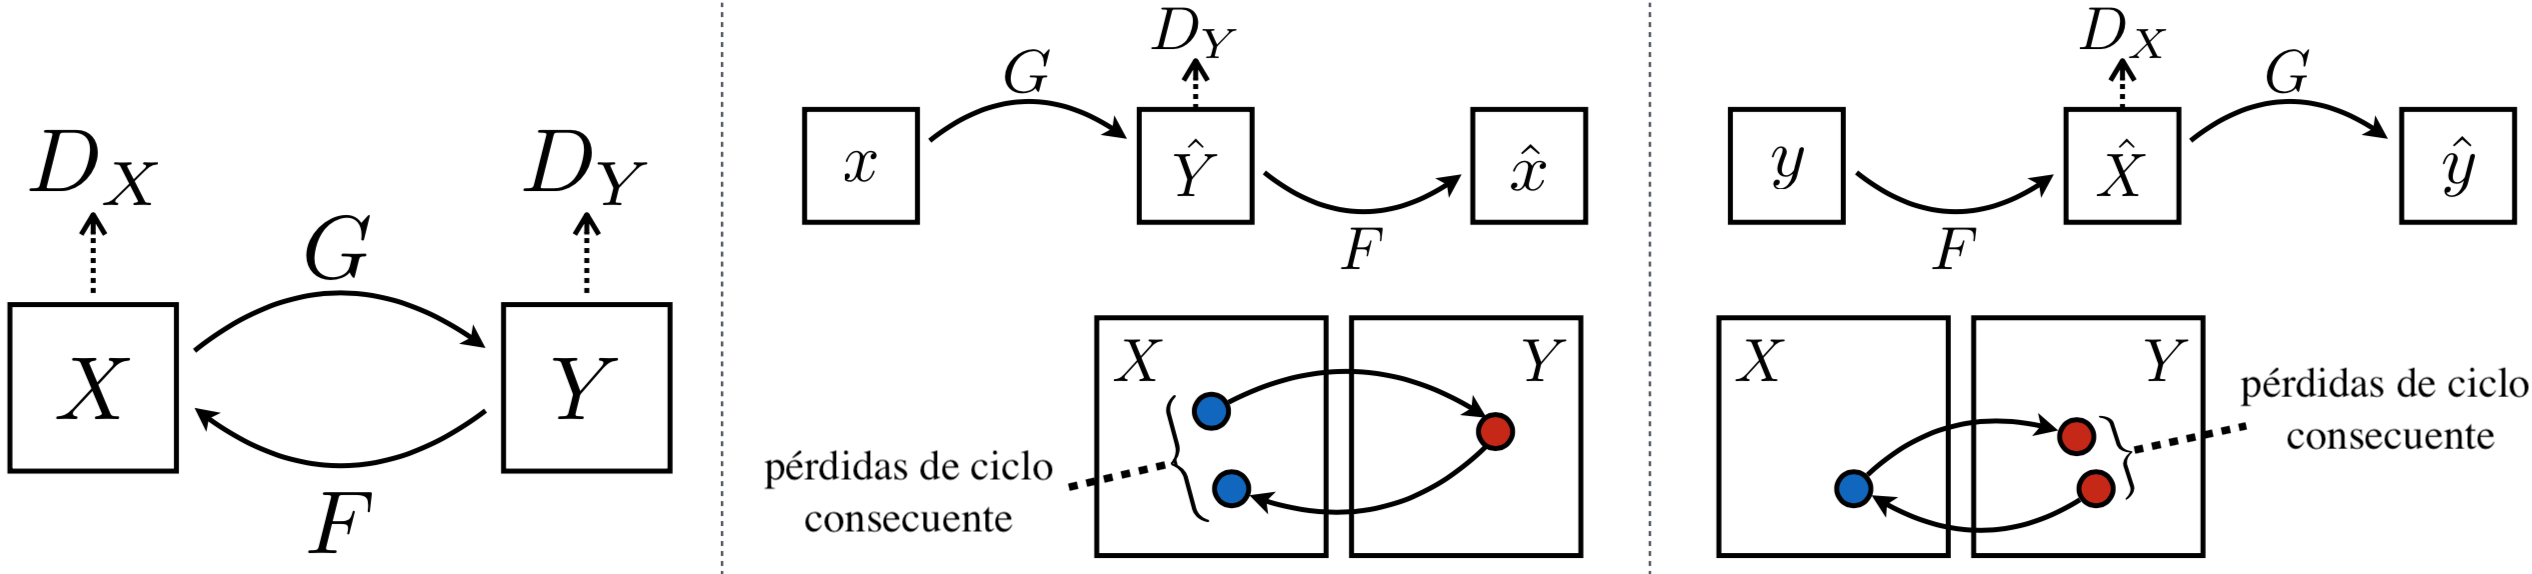
\includegraphics[width=\textwidth]{Images/cycleGAN.png}
    \caption{Estructura de los procesos de correspondencia directa ($G : X \to Y$) e inversa ($F : Y \to X$) en las Redes Generativas Antagónicas de Ciclo Consecuente \cite{cycleGAN}.}
    \label{fig:cycleGAN}
\end{figure}

En la \autoref{fig:cycleGAN} se puede observar la estructura simplificada de esta red, mientras que la expresión por la que se rige el aprendizaje es la siguiente:
\begin{align*}
    \underset{G,F}{min} \ \underset{D_X, D_Y}{max} \ \mathcal{V}(G, F, D_X, D_Y) &= \mathcal{L}_{GAN}(G, F, D_X, Y, X) + \mathcal{L}_{GAN}(G, F, D_Y, X, Y) \\ &\quad + \lambda \cdot \mathcal{L}_{cycleGAN}(G, F) \\
    \text{donde}~
    \mathcal{L}_{GAN} &\equiv \text{\autoref{eq:1}} \\
    \mathcal{L}_{cycleGAN}(G, F) &= \mathbb{E}_{x\sim p_{datos}(x)} \big[\norm{F(G(x)) - x}\big] + \mathbb{E}_{y\sim p_{datos}(y)} \big[\norm{G(F(y)) - y}\big] \\
    \lambda &\equiv \text{peso de la función de pérdidas de ciclo consecuente}
\end{align*}

En esta ocasión no sólo se pretende hacer que las imágenes generadas se perciban como las imágenes objetivo, sino que también las reconstruidas sean identificadas como las originales, garantizándose así la consistencia del ciclo. Es por ello que se introduce el término $\mathcal{L}_{cycleGAN}(G, F)$, el cual tiene en consideración el error existente entre las representaciones de entrada y sus reconstrucciones obtenidas al pasar a través de las dos funciones de mapeo, $G$ y $F$.

Resumidamente, en el ámbito particular de este proyecto, la utilización de estas redes tiene como fin el aumento del número de imágenes que tienen menor representación de la base de datos de expresiones faciales inicial para obtener un mejor comportamiento del sistema final.

\section{OpenCV}

OpenCV es una librería de código abierto de visión por computador con un fuerte enfoque en aplicaciones en tiempo real. Por este motivo y teniendo en cuenta su extendido uso, es la que se va a utilizar para el desarrollo del software encargado de detectar y capturar el rostro de forma periódica y en pseudo tiempo real para la posterior identificación de la expresión facial o, dicho de otra forma, para la confección del espejo inteligente.

La implementación de este sistema se va a llevar a cabo mediante Python y, dado que OpenCV fue diseñada para ser efectiva computacionalmente, en un sistema operativo GNU/Linux optimizado para el hardware de la Raspberry PI.

\begin{figure}
    \centering
    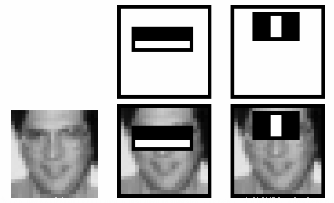
\includegraphics[scale=0.8]{Images/Haar.png}
    \caption{Características seleccionadas por AdaBoost. La primera característica mide la diferencia de intensidad entre la región de los ojos y la región superior de las mejillas, mientras que la segunda compara las intensidades de las regiones oculares con la del puente de la nariz \cite{Viola}.}
    \label{fig:Haar}
\end{figure}

En lo que respecta al procedimiento de la detección del rostro, este se va a realizar mediante clasificadores en casada basados en el efectivo método para detectar objetos propuesto por Paul Viola y Michael Jones en 2001 \cite{Viola}. Este método de aprendizaje automático consiste básicamente en entrenar una función cascada sobre numerosas imágenes positivas (imágenes con caras) y negativas (imágenes sin caras), extrayéndose los distintos atributos mediante las características Haar, tal y como se muestra en la \autoref{fig:Haar}. Su funcionamiento es similar a los filtros convolucionales vistos anteriormente, obteniéndose un único valor a partir de cada característica al restar la suma de los píxeles debajo del rectángulo blanco a la suma de los píxeles debajo del rectángulo negro. Sin embargo, la aplicación de estas operaciones a imágenes de altas resoluciones resulta muy costoso computacionalmente, por lo que se hace necesario utilizar métodos para disminuir el número de operaciones. Destacan el meta-algoritmo de aprendizaje automático Adaboost, que consigue optimizar la selección de características, y el método de la cascada de clasificadores, que aprovecha la hipótesis de que la mayor parte de los píxeles de una imagen son irrelevantes para agrupar la aplicación de las distintas características Haar en diferentes etapas de clasificación.
